\clearpage
\section{Prediction checks and consistent template visibility}
\label{sec:visibility-repair}

\paragraph{Fixed-action diagnosis.}
Replaying the original left-layout S trajectory reproduces all 256 actions and 257 sensor packets, matches 25 saved planning-score sets within $10^{-10}$, and reproduces the final native TSDF byte for byte. It performs no new route selection. The 31 original G/S planning states with one candidate and zero template gain occur after full coverage, when the remaining budget equals the shortest return cost. This is a return-budget effect, not evidence that early candidates prevent exploration.

Eight fixed reconstruction checkpoints separate predicted reward from acquired geometry. On actions 54--109, independently referenced correct surface area at 5~cm increases by 17.38~m$^2$ globally and 1.87~m$^2$ on the shelf; the cabinet loses 0.02~m$^2$. On 109--127, the respective net increments are 3.39, 0.06 and 0.57~m$^2$. These are Monte Carlo estimates over the fixed visible source reference, including gains and losses. They cannot be subtracted from weighted hypothetical-template reward as a calibration residual.

\paragraph{Visibility repair.}
The original gain removes free-space-contradicted reward samples but leaves their template triangles able to occlude other samples. Revision B2 changes only this visibility query. For an intersection $x$, let $z_f(x)$ and $d_f(x)$ denote its camera depth and valid measured depth at the nearest projected pixel in historical frame $f$. With the existing $\epsilon=0.10$~m,
\[
 F(x)=\bigvee_f[z_f(x)<d_f(x)-\epsilon],\qquad
 M(x)=\bigvee_f[d_f(x)-\epsilon\le z_f(x)\le d_f(x)+\epsilon].
\]
Only $F(x)\land\neg M(x)$ permits skipping an intersection. Only valid projections with finite positive measured depth enter these predicates; every preceding intersection is checked. Measured and unknown blockers remain opaque, and measured-TSDF occlusion is unchanged. This shared G/S revision retains templates, pseudo-posterior fitting, score weights, candidates, fusion and return rules. It does not correct template topology or feed free-space evidence into the fit posterior. The no-history arm still removes historical reward filtering, but retains this common visibility repair.

\paragraph{Prediction-to-measurement matching.}
A separately frozen evaluation-only replay captures original/repaired route-union weights on the same hypothetical points at actions 54 and 109. A point is source-supported when its distance to true source triangles is at most 5~cm; before/after reconstruction matching uses that same point and tolerance. No reference geometry reaches the actor. Table~\ref{tab:repair-prediction-match} retains both intervals. Of the newly restored weight, 0.998 and 1.483 are source-supported, unmatched before and matched after; these are weighted template-area units, not unique true square metres. A secondary nearest-source-point test yields 0.998 and 1.290. Restored weights also include 2.324 and 0.269 unsupported by source geometry. The repair recovers useful visibility, but these two fixed states retain substantial template mismatch and do not establish a causal endpoint or semantic advantage.

\begin{table}[!htbp]
\centering\small\setlength{\tabcolsep}{5pt}
\caption{Same-point diagnosis of two intervals on the original S route. Each pair is original/repaired. $W$ is weighted hypothetical-template area; source support is its weighted fraction within 5~cm of true triangles. Increment support uses only restored per-point weight. Overlapping hypotheses do not define unique true surface area. These are saved states, not new trials.}
\label{tab:repair-prediction-match}
\begin{tabular}{rrrr}
\toprule
Interval & $W$ (template units) & Source support (\%) & Increment support (\%) \\
\midrule
54--109 & 4.331 / 9.098 & 24.04 / 38.30 & 51.25 \\
109--127 & 1.436 / 3.283 & 51.76 / 70.71 & 85.43 \\
\bottomrule
\end{tabular}
\end{table}

\clearpage
% All 12 completed slots from the frozen B2 independent evaluation.
\begin{table}[!htbp]
\centering\small\setlength{\tabcolsep}{4pt}
\caption{All twelve visibility-repaired runs (B2). Definitions, sensing, action costs, 256-action allocation and fixed references are unchanged from Table~\ref{tab:dual-template-results}. Every row reaches 100\% correct-free reference coverage, records zero simulated collisions and returns to its initial pose. C stops at 130 actions; other arms use 256. This repeats the same two related layouts, not twelve new environments.}
\label{tab:visibility-repair-results}
\begin{tabular}{llrrrrrr}
\toprule
Layout & Arm & $A_{\rm end}$ & $A_{100}$ & Path (m) & F1 (\%) & $R_o$ (\%) & $R_c$ (\%) \\
\midrule
L & C & 130 & 67 & 22.4 & 91.92 & 73.69 & 49.26 \\
L & J & 256 & 88 & 42.0 & 92.76 & 82.17 & 88.71 \\
L & G & 256 & 97 & 42.8 & 92.63 & 82.61 & 83.79 \\
L & S & 256 & 97 & 42.8 & 92.63 & 82.61 & 83.79 \\
L & $S_{\rm no\ fit}$ & 256 & 97 & 43.2 & 92.38 & 83.46 & 85.87 \\
L & $S_{\rm no\ history}$ & 256 & 67 & 43.6 & 92.31 & 82.42 & 74.29 \\
\midrule
R & C & 130 & 66 & 22.4 & 92.43 & 70.80 & 70.04 \\
R & J & 256 & 100 & 43.2 & 92.60 & 81.09 & 79.21 \\
R & G & 256 & 100 & 43.2 & 92.60 & 81.09 & 79.21 \\
R & S & 256 & 100 & 43.2 & 92.60 & 81.09 & 79.21 \\
R & $S_{\rm no\ fit}$ & 256 & 100 & 43.2 & 92.60 & 81.09 & 79.21 \\
R & $S_{\rm no\ history}$ & 256 & 100 & 43.2 & 92.54 & 80.78 & 78.39 \\
\bottomrule
\end{tabular}
\end{table}


\begin{figure}[!htbp]
\centering
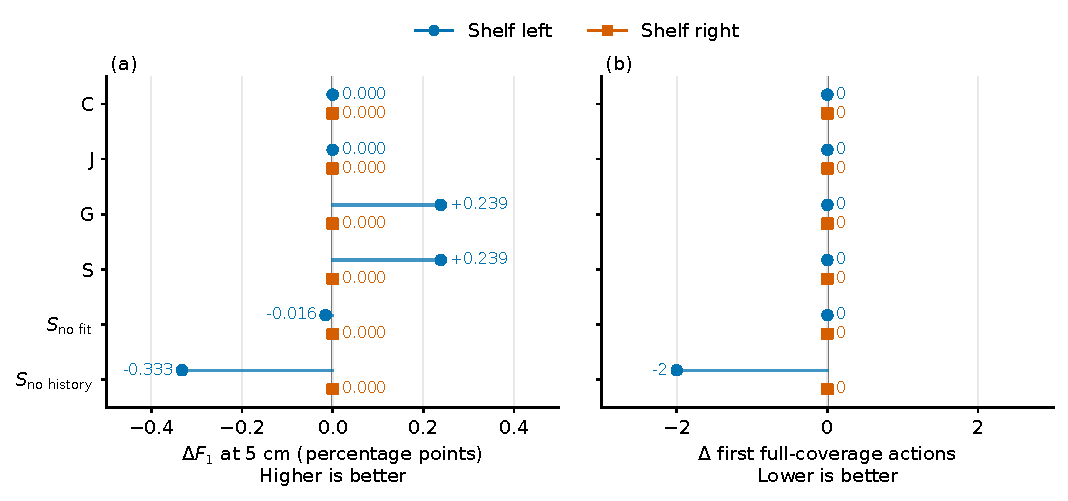
\includegraphics[width=\linewidth]{figures/B_to_B2_delta.pdf}
\caption{Paired B2 minus B changes for every arm and layout. Higher endpoint F1 and fewer actions to first full coverage are improvements. The two metrics use different checkpoints. These deterministic, related-layout comparisons do not support between-scene error bars.}
\label{fig:visibility-repair-change}
\end{figure}

\paragraph{Complete paired outcomes.}
G and S still have identical trajectories and native TSDF in both layouts. The repair increases left-layout F1 by 0.239 percentage points for both, without earlier full coverage; right-layout endpoints are unchanged. Left-layout S remains below J by 0.123 points at the same budget. S exceeds $S_{\rm no\ fit}$ by 0.254 points there but has lower recall on both target objects; the right layout ties. This does not establish a category benefit or generally improved target observation. The no-history arm triggers weighted point thinning in 22/14 planning states, so its mixed outcomes include a sampling effect. C/J retain their original complete trajectories. The 24 B/B2 runs reuse two related layouts. Earlier null results remain retained. Visibility consistency improves, but semantic exploration benefit remains unproven.
